\section{The cost of safety}

The advantage of using a VM to provide safety is that the necessary checks are easy to do, compared to native code, and most can be done at load-time. This leads to both a very modest increase in VM complexity due to the safety checks, and a lower run-time overhead. In this section we evaluate both.

% would be nice to get code size for Harbor and t-kernel.

\begin{table*}[]
 \centering
 \caption{Cost of safety guarantees}
 \label{tbl-safety-cost}
 \clearpage
\newgeometry{margin=1cm}
\thispagestyle{empty}
\begin{landscape}
\begin{table}[t!]
\caption{Cost of safety guarantees}
\label{tbl-safety-cost}
    \begin{tabular}{lrrrrrrrrrrrrrrr} % UPDATED 20180305
    \toprule
                                        & B.sort     &  H.sort    & Bin.Search & XXTEA      & MD5        & RC5        & FFT        & Outlier    & LEC        & CoreMark   & MoteTrack  & HeatCalib  & HeatDetect & \makebox[0.2mm]{} &   average \\
    \midrule
    \midrule
    \multicolumn{10}{l}{EXECUTED BYTECODE INSTRUCTIONS (\% of total executed bytecode instructions)} \\
    Array element/object field STORES   &       18.0 &        7.8 &        0.0 &        2.9 &        4.5 &        1.5 &        6.1 &        5.8 &        3.7 &        2.6 &       10.0 &        1.4 &        4.7 &                   &       5.3 \\
    Array element/object field LOADS    &       18.0 &       15.9 &        7.1 &        8.6 &        6.2 &        6.4 &        7.0 &       10.7 &        7.9 &       11.6 &       21.4 &        4.1 &        9.8 &                   &      10.4 \\
    \multicolumn{10}{l}{PERFORMANCE OVERHEAD VS NATIVE C (\% of native C)} \\
    unsafe                              &      101.2 &       88.5 &       65.2 &       57.6 &       45.7 &       19.5 &       17.7 &       75.7 &       84.6 &       97.0 &      156.3 &       30.5 &       73.4 &                   &      70.2 \\
    safe writes                         &      247.5 &      153.9 &       65.2 &       68.2 &       60.3 &       22.2 &       30.3 &      128.4 &      118.4 &      124.0 &      266.1 &       33.9 &       91.3 &                   &     108.4 \\
    safe reads and writes               &      393.9 &      287.8 &      151.7 &      100.0 &       80.3 &       33.4 &       43.0 &      226.6 &      179.8 &      202.2 &      445.1 &       43.9 &      126.9 &                   &     178.0 \\
    \multicolumn{10}{l}{PERFORMANCE OVERHEAD VS UNSAFE VM (\% of unsafe AOT)} \\
    safe writes                         &       72.7 &       34.7 &        0.0 &        6.7 &       10.0 &        2.3 &       10.7 &       30.0 &       18.3 &       13.7 &       42.8 &        2.6 &       10.3 &                   &      22.4 \\
    safe reads and writes               &      145.5 &      105.7 &       52.4 &       26.9 &       23.7 &       11.6 &       21.5 &       85.9 &       51.6 &       53.4 &      112.7 &       10.3 &       30.9 &                   &      63.3 \\
    \multicolumn{10}{l}{CODE SIZE OVERHEAD VS NATIVE C (\% of native C)} \\
    unsafe                              &      118.6 &      100.0 &      112.3 &       55.1 &       54.9 &      121.8 &        2.5 &      110.5 &       88.6 &       50.7 &      117.1 &      -17.2 &      107.7 &                   &      78.7 \\
    safe writes                         &      125.4 &      105.4 &      112.3 &       56.2 &       55.7 &      125.3 &        5.0 &      118.9 &       94.3 &       54.5 &      125.4 &      -16.4 &      114.7 &                   &      82.8 \\
    safe reads and writes               &      132.2 &      113.4 &      117.8 &       60.1 &       59.1 &      132.3 &        8.0 &      123.2 &      102.9 &       61.8 &      145.3 &      -13.9 &      118.5 &                   &      89.3 \\
    \multicolumn{10}{l}{CODE SIZE OVERHEAD VS UNSAFE VM (\% of unsafe AOT)} \\
    safe writes                         &        3.1 &        2.7 &        0.0 &        0.7 &        0.5 &        1.6 &        2.4 &        4.0 &        3.0 &        2.5 &        3.8 &        1.0 &        3.4 &                   &       2.3 \\
    safe reads and writes               &        6.2 &        6.7 &        2.6 &        3.2 &        2.7 &        4.7 &        5.4 &        6.0 &        7.6 &        7.4 &       13.0 &        4.0 &        5.2 &                   &       5.9 \\
    \bottomrule
    \end{tabular}
\end{table}
\end{landscape}
\clearpage
\restoregeometry

\end{table*}


\subsection{Run-time cost}
\label{sec-evaluation-run-time-cost}
\begin{figure}[]
  \centering
  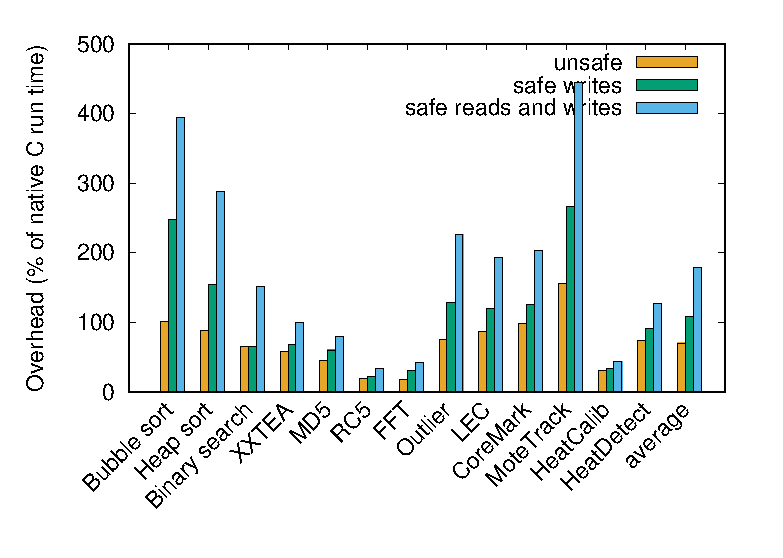
\includegraphics[width=0.6\linewidth]{safety-cost.eps}
  \caption{Overhead increase due to safety checks}
  \label{fig-safety-cost-per-benchmark}
\end{figure}

\begin{figure}[]
   \centering
  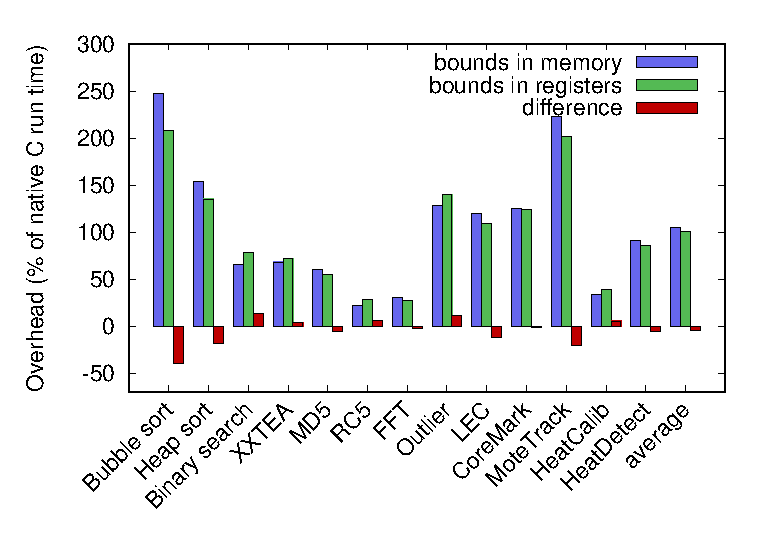
\includegraphics[width=0.6\linewidth]{safety-cost-diff-using-regs.eps}
  \caption{Comparison of safety cost with bounds in memory or registers}
  \label{fig-safety-cost-memory-or-registers}
\end{figure}

First we examine the run-time cost of our safety guarantees. We use 8 benchmarks, 7 smaller ones and the larger CoreMark benchmark \cite{coremark} which consists of several functions, implementing a state machine, linked list processing, and several matrix operations. All benchmarks are implemented in both C and Java, with the Java implementation following the original C code as closely as possible. We then compare the running times for both versions and report the overhead, presented as a percentage of the optimised native C runtime, i.e. a 100\% overhead corresponds to a run time for the Java version that is twice as long as the corresponding C implementation.

Table \ref{tbl-safety-cost} shows the results for our 8 benchmarks. Figure \ref{fig-safety-cost-per-benchmark} shows the data in the first section of the table. The baseline is the unsafe version of our VM, which is on average 69\% slower than native C. When we add our safety checks this overhead increases to 98\%, corresponding to an 18\% increase in runtime compared to the unsafe VM.

We can see the cost of safety depends greatly on the benchmark we run. Most checks are done at load-time, including writes to local and static variables. The only check that adds significant run-time overhead is check \ref{chk-memory-access-within-heap}, which checks the target of an object field or array write is within the heap bounds.

Thus, the run-time overhead is determined by the number of object or array writes a benchmark does. Bubble sort has the highest increase in running time as a result of these checks at 47\%, while binary search, which does no writes at all is unaffected. CoreMark, being a large benchmark with a mix of operations, is close to the average slowdown.

\paragraph{Safe reads}
Next we consider read safety. Up to this point our VM only checks the application cannot \emph{write} to memory it's not supposed to write to, however, it may still read from any location.

The recently published Meltdown and Spectre vulnerabilities in desktop CPUs can be exploited by malicious code to read from anywhere in memory, exposing both kernel's and other applications private data, which may contain sensitive information such as authentication tokens, passwords, etc. This sent OS vendors rushing to release patches, which early report suggest may cause a performance penalty of 5-30\% \cite{register-spectre-meltdown}.

Whether this is also a problem on a sensor node depends on the scenario. If the VM or other tasks contain sensitive information, then this obviously needs to be protected. However, in many sensor node applications the node may only be running a single application, and our VM does not contain any state that would be useful to an attacker. In these cases, only providing write safety will be sufficient.

Adding read safety to our VM is trivial: instructions to read from local and static variables is already protected since these instructions reuse the same code to access them as the instructions to write to them. For heap access, we simply add the same call to \mycode{heapcheck} to the \mycode{GETARRAY} and \mycode{GETFIELD} just before the actual read.

Looking at Figure \ref{fig-safety-cost-per-benchmark}, we see the cost of providing read safety is higher than write safety. Most applications read from an array or object much more frequently than they write to them. As a result, our VM with read and write safety turned on slows down by roughly 50\% on average, corresponding to a 152\% slowdown over native C. The per benchmark picture is similar to that of write-only safety with bubble sort, which spends almost all it's time reading and writing from and to arrays, being the worst hit, while rc5 is still only 33\% slower than C. Again, CoreMark performs very close to the overall average.

\paragraph{Keeping heap bounds in registers}
In Section \ref{sec-safety-heap-access} we considered several alternatives to our chosen heap bounds check, one of which was to keep the bounds in dedicated registers to avoid having to fetch them from memory for each check. Here we evaluate this choice.

The expected performance for this alternative is easily calculated. Having the bounds in registers would reduce the cost of the check from 22 to 14 cycles, reducing the safety overhead by 36\%. However, we would have 4 registers less to use for stack caching. We ran our experiments a second time for our unsafe VM, this time reducing the number of registers available to the stack cache by 4. Since this doesn't affect the number of heap accesses, we then added the observed overhead for safety checks, reduced by 36\%.

Figure \ref{fig-safety-cost-memory-or-registers} shows the overhead for our chosen approach with the heap bounds in memory, compared to the expected overhead is we keep the heap bounds in registers. For some benchmarks such as bubble sort, the savings in heap bounds checks outweighs the reduced effectiveness of the stack cache, But the improvement in performance is rather small at 20\%, and other for benchmarks the reverse is true, with binary search overhead increased by 35\%. Overall the benchmarks were nearly perfectly balanced on average, as was the larger CoreMark benchmark.

As future work we may consider using some basic statistics, such as the percentage of array write instructions and average stack depth, to choose one of the two options on a per-method basis. But as usual there is a tradeoff, in this case VM size and complexity, and our calculations show that even choosing the best option for each of the smaller benchmarks only reduces overhead by a few percent.

\subsection{Code-size cost}
Next, we examine the cost of safety in terms of code size. This comes in two parts: increase VM complexity and size, and the increase in the code it generates.

Most of our checks are not more complex than comparing two integers, and failing if a condition is not met. The most complex part is deciding the stack effects of instructions to guard against stack over- or underflow. This comes in the form of a table that encodes the effects of most instructions, and some specialised code to analyse a handful of instructions without fixed effect. In total, the increase in VM size for our safe version is a modest 1776 bytes.

As we can see in Table \ref{tbl-safety-cost}, the size of the code the VM generates increases by only 1.6\%. Since most checks occur at load-time, most instructions produce exactly the same native code in the safe version of our VM. The exceptions are \mycode{INVOKEVIRTUAL} and \mycode{INVOKEINTERFACE}, which now contains the expected stack effects to realise check \ref{chk-invokevirtual-stack-effects-match}, and the array and object write instructions \mycode{PUTFIELD} and \mycode{PUTARRAY}, which now emit a single extra \mycode{CALL} instruction the \mycode{heapcheck} routine. Since these instructions are both relatively rare, and already generate a larger block of native instructions than most instructions do in the unsafe version, the total effect on code size is very limited.

\subsection{Comparison to native code alternatives}
As discussed in Section \ref{sec-state-of-the-art-safety}, several non-VM approaches exist to guarantee safety on a sensor node. Two of these, \emph{t-kernel} and Harbor, allow the node to guarantee safety independent of the host. In this section we compare these to our approach, and consider the question whether a VM is a good way to provide safety.

\emph{t-kernel} reports a slowdown of between 50 and 200\%, which is roughly in the same range as our VM. However both \emph{t-kernel} and our approach provide additional advantages. In \emph{t-kernel}'s case a form of virtual memory, and for our VM platform independence. This makes them hard to compare, but we note that while the performance of both systems is similar, t-kernel's code size overhead is much larger at a 6-8.5x increase, limiting the size of programmes we can load onto the device.

A better comparison is possible for Harbor, which only provides safety. The overhead reported is in the range of 160 to 1230\%. The latter is for a synthetic benchmark, filling a block of memory with arbitrary data. The authors note this simulates a very common behaviour of sensor network applications: copying sampled sensor data into a buffer that can be transmitted into the network.
% TODO in thesis, expand this with worst case on method calls

We implemented this as a benchmark that fills an array of 256 elements with an arbitrary number. This is one of the worst cases for our VM since consecutive array writes are expensive for two reasons: (i) in our VM this results in repeated executions of the \mycode{PUTARRAY} instruction, which calculates the target address for each write, while native code can slide a pointer over the array, eliminating the need for repeated address calculations. (ii) each of these writes will trigger a call to \mycode{heapcheck}.

Our benchmark is implemented as a simple loop as shown in Listing \ref{lst-fill-array}.

\begin{listing}[H]
	\centering
 	\begin{minted}{java}
        for (short i = 0; i < NUMNUMBERS; i++) {
            numbers[i] = (byte)1;
        }
	\end{minted}
	\caption{Fill array benchmark (8-bit version)}
	\label{lst-fill-array}
\end{listing}

\begin{table}[]
 \centering
 \caption{Overhead for the fill array benchmark as a percentage of native C}
 \label{tbl-fill-array-results}
\begin{tabular}{lrrr}
\toprule
%benchmark & unsafe overhead & safe overhead \\
%\midrule
%8-bit  byte  & 210\% & 566\% \\
%16-bit short & 182\% & 452\% \\
%32-bit int   & 155\% & 336\% \\
Benchmark & Unsafe & Safe & Increase due to \\
 & overhead & overhead & safety checks \\
\midrule
8-bit  bytes  & 210\% & 566\% & 356\% \\
16-bit shorts & 182\% & 452\% & 270\% \\
32-bit ints   & 155\% & 336\% & 181\% \\
\bottomrule
\end{tabular}
\end{table}

The resulting overhead is shown in Table \ref{tbl-fill-array-results}. We implemented our benchmark for arrays of bytes, shorts and ints. Unfortunately the Harbor paper does not mention the size of elements in their buffer, nor whether this will make a difference for their overhead. For our VM, the worst case is filling a byte array because here the relative overhead from address calculation and safety checks is highest.

The worst case overhead due to safety checks is 356\%, considerably less than Harbor's 1230\%, and dropping to 181\% when storing ints instead of bytes. Our VM also incurs other overhead, not related to safety checks, but the total overhead of 566\% in the worst case is still less than half of Harbor's.

While our VM is currently faster than Harbor, the comparison is not entirely fair. Harbor lists the cycle overhead for all of it's 5 run-time protection primitives. We assume that without any function calls, only the 'Write access check' is relevant to this benchmark, which takes 65 cycles. In contrast, our \mycode{heapcheck} routine only takes 22 cycles.

The difference is due to Harbor's more fine grained protection, which allows it to grant access to any aligned block of 8 bytes to the application, while our VM is more coarse. If Harbor could be modified to use a check similar to ours, it's overhead could potentially be reduced to $1230 / 65 * 22 \approx 416\%$. This puts it in the middle of our three versions in terms of total overhead. However, it is not clear from the paper whether Harbor's architecture could support such a coarse-grained check since it requires all application data that needs run-time write checks to be in a single segment.

% While this shows our approach achieves a performance comparable to even an optimised version of Harbor, it does not highlight the advantage of using a VM to provide safety since both approaches much check each write to an array. However, our approach can verify writes to local and static variables to be safe at translation time, eliminating the need for a run-time check, while we can tell from the Harbor sources \cite{sos-operating-system-source} that its verifier requires \emph{all} stores to go through its write access check.

% This means our approach should have a distinct advantage for code with frequent writes to local variables. The Harbor paper also contains an FFT benchmark, and in the source code we find a copy of the same fixed point FFT algorithm used in our benchmark, albeit in a 16-bit version while our benchmark uses the 8-bit version. In Harbor's case this results in an overhead of 380\%, while our VM is significantly faster at only 145\%.



%TODO: figure this out: if we do the same /65*22 on this 380 performance, Harbor is only 128\% slower, beating our 145\%...
%TODO: say something about Harbor's claim to reduce checks at the cost of more complexity
